\documentclass[11pt, titlepage]{article} 

\usepackage[utf8]{inputenc}

\usepackage{geometry} 
\geometry{a4paper}

\usepackage{graphicx}
\usepackage{mathtools}
\usepackage{paralist}
\usepackage{verbatim} 
\usepackage{subfig}
\usepackage[affil-it]{authblk}
\usepackage{gensymb}
\usepackage{listings}
\usepackage{color}

\usepackage{fancyhdr}
\pagestyle{fancy}

\renewcommand{\headrulewidth}{0pt} 
\lhead{}\chead{}\rhead{}
\lfoot{}\cfoot{\thepage}\rfoot{}

\usepackage{sectsty}
\allsectionsfont{\sffamily\mdseries\upshape}

\usepackage[notlof,notlot]{tocbibind}
\usepackage[titles,subfigure]{tocloft} 
\renewcommand{\cftsecfont}{\rmfamily\mdseries\upshape}
\renewcommand{\cftsecpagefont}{\rmfamily\mdseries\upshape}

\definecolor{dkgreen}{rgb}{0,0.6,0}
\definecolor{gray}{rgb}{0.5,0.5,0.5}
\definecolor{mauve}{rgb}{0.58,0,0.82}

\lstset{frame=tb,
  language=Java,
  aboveskip=3mm,
  belowskip=3mm,
  showstringspaces=false,
  columns=flexible,
  basicstyle={\small\ttfamily},
  numbers=none,
  numberstyle=\tiny\color{gray},
  keywordstyle=\color{blue},
  commentstyle=\color{dkgreen},
  stringstyle=\color{mauve},
  breaklines=true,
  breakatwhitespace=true,
  tabsize=3
}

\title{Alternative Sources of Energy}
\author{Filip Cima}
\affil{Vysoká Škola Báňská - Technická Univerzita Ostrava}
\date{\today}

\begin{document}
\maketitle

\newpage

\tableofcontents

\newpage

\section{Introduction}

	There are five general ways to obtain electricity besides nuclear, thermal power stations and from other, non-renewable sources.
	\newline
	\textbf{These are:}
	\begin{enumerate}
		\item{Solar energy}
		\item{Hydropower}
		\item{Geothermal energy}
		\item{Wind energy}
		\item{Solar energy}
	\end{enumerate}

	In following sections we will focus on describing each type of energy and later in the document we will pay attention to explaining how a wind turbine works and how a community can be self sufficient in energy industry.
	\pagebreak
\section{Major types}
	\subsection{Solar Energy}
		Solar power is the conversion of sunlight into electricity using photovoltaic effect (explanation)
		It is the most common alternative source of energy you can install at home.
		It is also used for warming water up, making electricity, drying clothes, heating up homes. People think that it's the best thing going from an enviromental perspective.
		\vspace{0.5cm}
		\begin{figure}[!h]
			\begin{center}
				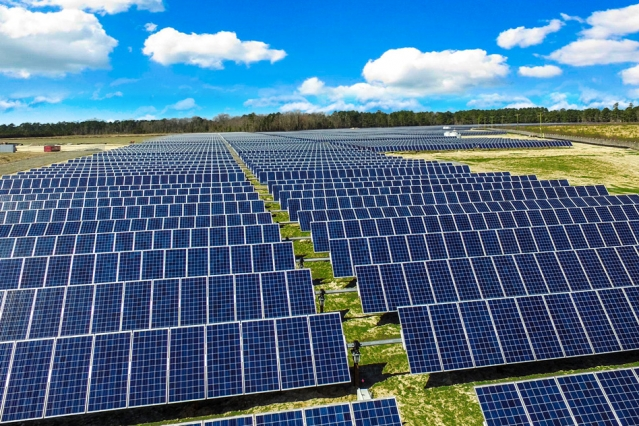
\includegraphics[height=4cm]{img/solar_panels.jpg}
				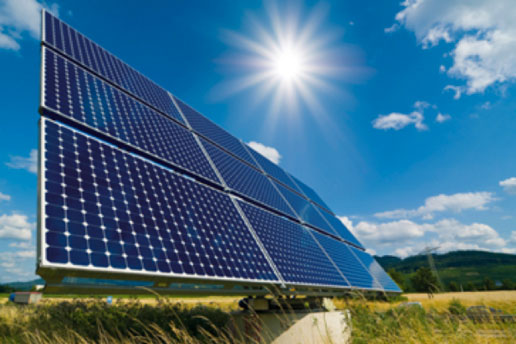
\includegraphics[height=4cm]{img/solar_panels_2.jpg}
				\caption{Solar panels at MIT university.}
				\label{obr.graphicx}
			\end{center}
		\end{figure}

		\subsubsection{Photovoltaic}
			Photovoltaic solar technology directly converts sunlight into electricity using panels made of semiconductor cells. These are the panels we can find on roofs of houses more and more often.

		\subsubsection{Solar}
			This type captures the sun’s heat. This heat is used directly or converted into mechanical energy and in turn electricity, known as concentrated solar power . This heat is used directly (low‑temperature solar thermal) or converted into mechanical energy and in turn electricity (concentrated solar power – CSP).

	\subsection{Hydropower}
		Hydroelectric power generates about 10 \% of US energy. Flowing water creates energy that can be captured and turned into electricity. 
		\newline
		The most common type of hydroelectric power plant uses a dam on a river to store water in a reservoir. Water released from the reservoir flow through a turbine, spinning it, which in turn activates a generator to produce electricity.
		\newline
		There are more types of hydroelectric power plants - for example pumped storage plant, which can even store power.
		\newline
		\newline
		\textbf{Advantages:}
		\begin{itemize}
			\item Dams are designed to last many decades.
			\item Lake's water can be used for more purposes.
			\item Water can be stored if there's not much energy needed.
		\end{itemize}

	\subsection{Geothermal energy}
		\begin{figure}[!h]
			\begin{center}
				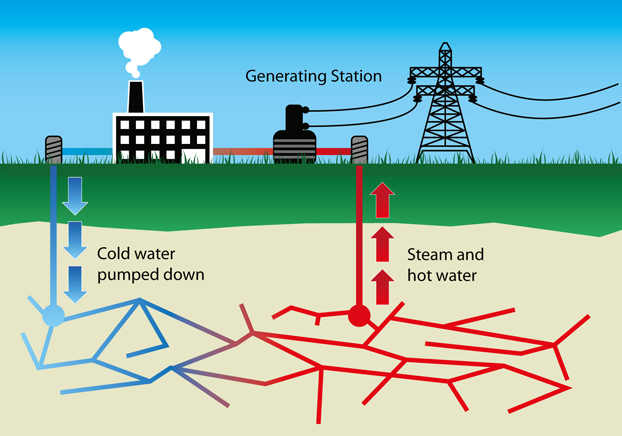
\includegraphics[height=10cm]{img/geothermal_energy.png}
				\caption{Geothermal plant.}
			\end{center}
	\end{figure}

		\textbf{Geothermal energy} is heat energy generated and stored in the Earth. Thermal energy is the energy that determines the temperature of matter. The geothermal energy of the Earth's crust originates from the original formation of the planet and from radioactive decay of materials \textit{(in currently uncertain but possibly roughly equal proportions)}. The geothermal gradient, which is the difference in temperature between the core of the planet and its surface, drives a \textbf{continuous conduction of thermal energy} in the form of heat from the core to the surface.

		\vspace{0.5cm}
		We distinguish \textbf{three basic types of geothermal energy}:
		\newline


		\begin{itemize}
			\item \textbf{Liquid-dominated plants}
			\begin{itemize}
				\item more common with temperatures above 200 \degree C
				\item found near young volcanoes surrounding Pacific Ocean
				\item generates around 2-10 MWe
			\end{itemize}
			\item \textbf{Thermal energy}
			\begin{itemize}
				\item water can be piped from geysers directly into radiators
				\item Iceland is the world leader in direct applications of thermal energy
			\end{itemize}
			\item \textbf{Enhanced geothermal systems}
			\begin{itemize}
				\item EGS actively inject water into wells to be heated and pumped back out.
				\item zero environmental damage
				\item small scale EGS can be seen in France, Germany
			\end{itemize}
		\end{itemize}


	\subsection{Wind energy}

		\textbf{Wind power} is the use of air flow through wind turbines to mechanically power generators for electric power. Wind power, as an alternative to burning fossil fuels, is \textbf{plentiful}, \textbf{renewable}, \textbf{widely distributed}, \textbf{clean}, produces \textbf{no} greenhouse gas \textbf{emissions} during operation, \textbf{consumes no water}, and uses little land. The net \textbf{effects on the environment are far less problematic than those of nonrenewable power sources}.



		\subsubsection{Wind farms}
			A \textbf{wind farm} is a group of wind turbines in the same location used for production of electric power. A large wind farm may consist of \textbf{several hundred individual wind turbines} distributed over an extended area, but the land between the turbines may be used for agricultural or other purposes. For example, Gansu Wind Farm, the largest wind farm in the world, \textbf{has several thousand turbines}. A wind farm may also be located offshore.
			\newpage
			\textbf{Large onshore wind farms:}
			\newline

			\begin{tabular}{|l|l|c|}
			  	\hline
				\bf{Wind Farm}&\bf{Country}&\bf{Current capacity}\\
				\hline
				Gansu Wind Farm & China & 6,800 MW\\
				Muppandal Wind Farm & India &1,500 MW\\
				Alta & United States   &1,320 MW \\
				Jaisalmer Wind Park & India & 1,064 MW\\
				\hline
			\end{tabular}

			\subsection{Self sufficient country in energy}
			In our english text book we have a picture showing a little electricity-independent town.
			\newline
			Look at the picture below and think about its implementation in real life. Is this even possible?

			\begin{figure}[!h]
				\begin{center}
					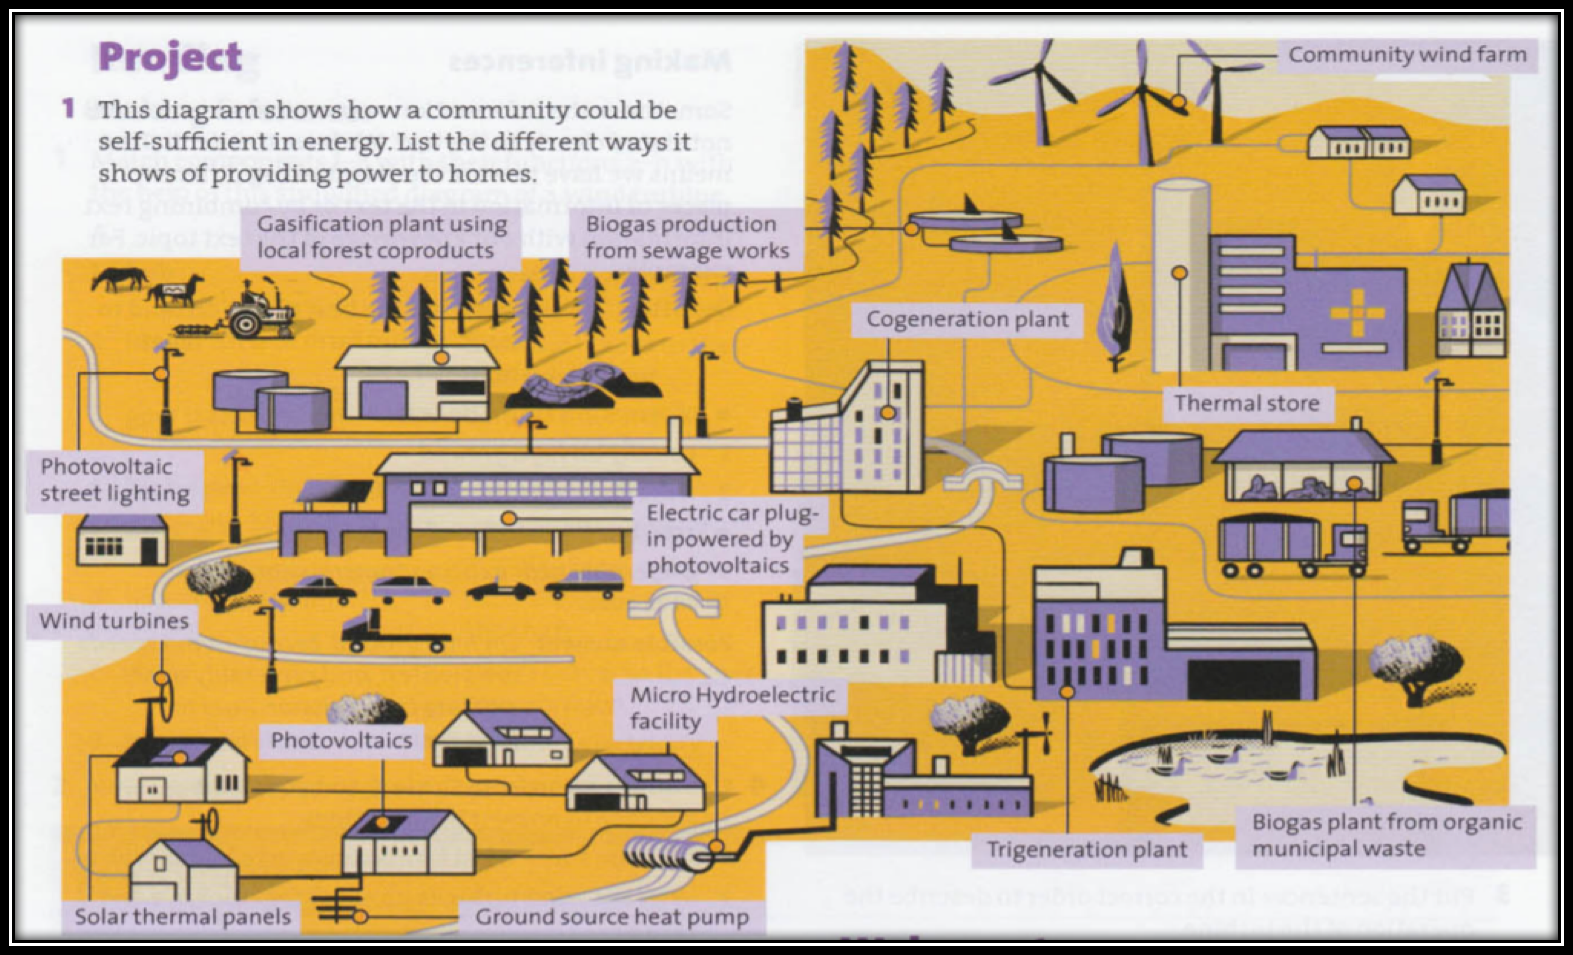
\includegraphics[height=9cm]{img/textbook.png}
					\caption{Textbook example of a self sufficient community.}
				\end{center}
			\end{figure}

			\pagebreak

\section{Something more to add}
	\subsection{Can we have code snippets in \LaTeX?}
		\textbf{Hell yeah!}

		\begin{lstlisting}
// Hello LaTeX!
public static void main() {
	System.out.println("Hello from TEX!");
	
	for(int i = 0; i < 3; i++) 
		System.out.println("Supercool!");
}
		\end{lstlisting}

	\subsection{How about math formulas?}
		\textbf{No problem, boss.}
			\subsubsection{Arrays}
				Arrays of mathematics are typeset using one of the matrix environments as in
				\[
					\begin{bmatrix}
						1 & x & 0 \\
						0 & 1 & -1
					\end{bmatrix}\begin{bmatrix}
						1  \\
						y  \\
						1
					\end{bmatrix}
					=\begin{bmatrix}
						1+xy  \\
						y-1
					\end{bmatrix}.
				\]

				Many arrays have lots of dots all over the place as in
				\[
					\begin{matrix}
						-2 & 1 & 0 & 0 & \cdots & 0  \\
						1 & -2 & 1 & 0 & \cdots & 0  \\
						0 & 1 & -2 & 1 & \cdots & 0  \\
						0 & 0 & 1 & -2 & \ddots & \vdots \\
						\vdots & \vdots & \vdots & \ddots & \ddots & 1  \\
						0 & 0 & 0 & \cdots & 1 & -2
					\end{matrix}
				\]
\end{document}
